\chapter{Core Mechanics}

This chapter describes the core mechanics of Rise.

\section{Defining the Undefined}
    This book does not attempt to include specific rules for every aspect of a realistic world.
    Unless defined otherwise - or if it's not worth the effort to look up Rise's exact rules in the flow of a game - you should assume that the universe works more or less like the real world does, and as long as everyone agrees that something is reasonable, it's not worth worrying about in more detail.

    For example, Rise does not have specific rules for how long it takes to eat a meal, the arc that a thrown ball takes through the air, or how much extra weight a well-made chandelier can hold without breaking.
    It's possible to imagine situations where each of those might be important to a game, however, so you'll have to guess what would be reasonable as obscure situations arise.
    The Game Master has the final word when defining ambiguities like this.

    \subsection{Resolving Ambiguity}\label{Resolving Ambiguity}
        When the rules are ambiguous about how they apply to you and no other creature, you decide how to resolve that ambiguity.
        For example, if an ability causes you to remove one of your \glossterm{vital wounds}, and you have more than one vital wound, you choose which vital wound is removed.
        When the rules are ambiguous in any other situation, the GM decides how to resolve that ambiguity.
        This includes situations where multiple creatures are relevant and situations where no particular creature is relevant.

\section{Making Checks}\label{Checks}\label{Making Checks}
    Checks are required to perform actions that have a chance of failure where the difficulty is not measured by the defense of another creature or object.
    For example, climbing a wall or remembering an obscure piece of trivia may require a check.

    To make a check, roll 1d10 and add your modifier with the check.
    You compare that result to a \glossterm{difficulty value} that represents the difficulty of the task.
    The more difficult the task, the higher the \glossterm{difficulty value} will be.
    If your result is equal to or higher than the \glossterm{difficulty value}, the check succeeds.
    This usually means you accomplish a task successfully.
    Otherwise, the check fails.
    This usually means that nothing happens, though sometimes there are specific consequences for failure.

    \subsection{Critical Success}
        If your check result is at least 10 higher than the \glossterm{difficulty value}, your check is a \glossterm{critical success}.
        Some checks have a special effect on a critical success.
        For example, a critical success while climbing means you move twice as quickly (see \pcref{Climb}).

    \subsection{Standard Difficulty Values}\label{Standard Difficulty Values}
        Most checks are made against a fixed \glossterm{difficulty value} that represents how hard the task is.
        Detailed rules for determining difficulty values in specific circumstances can be found in the Expanded Skills chapter from the Tome of Guidance.
        However, most of the time, it's not worth the effort to consult charts and tables to figure out how hard a task is.
        Instead, you can estimate it based on the guidelines below.

        \begin{itemize}
            \item DV 0 - Easy: Only an exceptionally incompetent or impaired person could possibly fail a DV 0 check. For example, this includes walking on rough ground without tripping (Balance) or noticing that a yelling, red-faced person is angry (Social Insight).
            \item DV 5 - Average: A typical human with no relevant skills should still succeed at a DV 5 check without much issue. However, it would be possible to fail in a stressful situation where time is limited if the person had no relevant training. For example, this includes climbing a ladder (Climb) or hearing the topic of a nearby conversation in a crowded bar (Awareness).
            \item DV 10 - Hard: A typical human with no relevant skills might succeed at a DV 10 check, but only if they were very lucky or had a lot of time on their hands. An experienced practioner might fail infrequently in stressful circumstances, but a world-class expert would never fail. For example, this includes swimming in fast-moving water (Swim) or providing first aid to mitigate a barely lethal wound (Medicine).
            \item DV 15 - Very Hard: Only an experienced practioner could succeed at a DV 15 check, and they would still need to get lucky if they were in a rush. Even a world-class expert at the peak of real-world human potential could fail, but only rarely. For example, this includes picking a well-made lock (Devices) or holding your breath for eight minutes while staying still (Endurance).
            \item DV 20 - Almost Impossible: A world-class expert like an Olympic medalist could succeed at a DV 20 check if they were lucky or patient. Succeeding consistently at tasks of this difficulty requires superhuman capabilities. For example, this includes climbing a weathered natural rock wall without equipment (Climb) or squeezing through a space with a diameter of only half a foot (Flexibility).
            \item DV 25\add - Impossible: No real-world human can succeed at a DV 25 check. This sort of feat is only possible for high-level Rise characters who have explicitly surpassed ordinary limitations. For example, this includes running at full speed along a slack rope (Balance) or climbing a sheer glass pane (Climb).
        \end{itemize}

    \subsection{Trying Again}
        You can think of checks as being broadly divided into two categories: checks that give you information, and checks that cause a change in the world around you.
        In general, you can retry checks that change your environment indefinitely until you succeed.
        The only major limiting factor to those checks is that failure sometimes also changes your environment in ways that may punish your failure or make it impossible to retry the check.
        For example, if you are trying to climb a cliff, you can keep trying until you succeed, but you may take falling damage from falling off while halfway up the cliff.

        You generally cannot retry checks that give you information unless the situation changes in a way that is relevant to your check.
        This often takes the form of giving you new information.
        For example, if you've already examined a creature to determine whether they are disguised, you can't keep just keep staring that creature to make sure.
        However, if you splash the creature with water which washes away some makeup, you can try again now that you have more information.

        % TODO: it would be nice if this wasn't necessary
        In addition, checks that require a free action to make can never be made more than once for the same purpose within a round.

    \subsection{Opposed Checks}
        An opposed check involves multiple creatures competing to get the highest result.
        In case of a tie, all tied creatures roll again to break the tie.
        Usually, the creature with the highest result succeeds, while all other creatures either fail completely or simply succeed less effectively depending on the situation.

        Some opposed checks involve multiple creatures using the same skill to see who does the best job.
        For example, a climbing race up a wall might involve each participant rolling a Climb check, or you might make a Strength check to hold a door closed while another creature tries to shove it open.
        Alternately, it can involve creatures rolling opposite skills.
        For example, if you are trying to hide, you roll a Stealth check opposed by the Awareness check of any creatures who could notice you.

        Not all opposed checks require all participants to roll at the same time.
        For example, a creature who creates a disguise rolls the Disguise check at the time that the disguise is created.
        A creature who tries to notice the disguise would roll their Awareness check at the time they see the disguised creature.

    \subsection{Hidden Checks}
        The GM can always make checks on your character's behalf without telling you.
        Generally, this is used for observation-based skills.
        For example, it's very suspicious if the GM tells you to make an Awareness check and then tells you that you don't see anything interesting.
        One of the ways a GM can avoid that is by simply rolling a check on behalf of your character and only telling you the result if you succeed.

    \subsection{Group Checks}
        When multiple characters are trying to make the same check simultaneously, they may be able to work together.
        There are two kinds of group checks.

        \parhead{Collaborative Checks} When making a collaborative check, each member of the group gets their own result. Collaborative checks might include a group of scouts sneaking up on an enemy camp, a group of adventurers climbing a cliff, or a group of spies lying about their true allegiances.

        When making a collaborative check, the group must choose a leader before making the check.
        Each member of the group can make the check using the higher of their check modifier and half the leader's check modifier. Other modifiers apply normally.

        The group leader must remain in a position to help the other members of the group for the group members to gain this benefit. For example, if a group is making a collaborative check to leap across a chasm, the leader must jump last. If the group is making a collaborative Stealth check, the leader must remain adjacent to the other members of the group to prevent their mistakes quietly. The exact circumstances depend on the situation.

        \parhead{Collective Checks} The group works together to get a single result. Collective checks might include a group of diplomats persuading a noble to go to war, a group of medics tending to a dying warrior, or a group of scouts keeping watch for enemy attacks.

        When making a collective check, the group uses the highest result from any character making the check.
        In addition, that character gains a \plus1 bonus for each other character who also attempted the check, as long as their check result was no more than 5 points lower than the check's difficulty value.

        \parhead{Making Group Checks} A group check is not always possible. If the whole group is leaping over a chasm at once to escape a dragon, there is not enough time to designate a leader and have them aid the others to make a collaborative check. In general, a group check is only possible if the group has at least five rounds to work together, though this time may vary widely depending on the situation and the check being made.

\section{Resting}\label{Resting}
    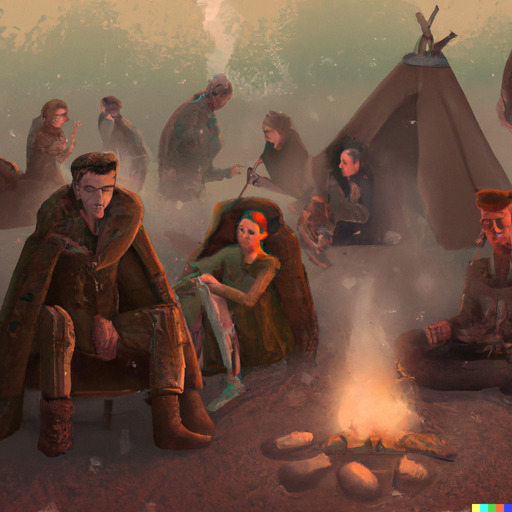
\includegraphics[width=\columnwidth]{core mechanics/resting}

    When you have a moment to relax, you can rest to regain some of your expended resources.
    There are two main types of rests: a \glossterm{short rest} and a \glossterm{long rest}.
    Resting is not actually an ability in the same sense as most other abilities.
    You do not declare that you are using the ``short rest'' ability, and you do not have to differentiate between whether you intend to take a short rest or a long rest.
    The benefits of taking a short rest or long rest happen automatically after you spend enough time avoiding strenuous activity.
    Resting at night is often combined with sleeping, but you can rest at any time without sleeping.

    % TODO: clarify interrupted rests

    \subsection{Short Rest}\label{Short Rest}
        Resting for ten minutes is considered a \glossterm{short rest}.
        When you finish a short rest, you gain the following benefits.
        \begin{itemize}
            \item Your \glossterm{hit points} become equal to your maximum hit points.
            \item Your current \glossterm{damage resistance} becomes equal to your maximum damage resistance.
            \item You regain any \glossterm{attunement points} you released from \glossterm{deep attunement} effects (see \pcref{Deep Attunement}).
            \item You remove all \glossterm{conditions} affecting you (unless they cannot be removed normally).
            \item Some other abilities have specific effects that last until you finish a short rest.
        \end{itemize}

    \subsection{Long Rest}\label{Long Rest}
        Resting for eight hours is considered a \glossterm{long rest}.
        When you finish a long rest, you gain the following benefits.
        \begin{itemize}
            \item You remove one of your vital wounds (see \pcref{Removing Vital Wounds}).
                The Medicine skill can increase this healing (see \pcref{Accelerate Recovery}).
            \item Your \glossterm{fatigue level} becomes 0.
            \item Some other abilities have specific effects that last until you finish a long rest.
        \end{itemize}

        You can take multiple long rests consecutively to recover from extensive vital wounds.

    \subsection{Sleep and Fatigue}\label{Sleep and Fatigue}
        A typical creature needs a minimum of 6 hours of sleep for every 18 hours spent awake, and a minimum of 50 hours of sleep every week.
        You can stay awake beyond those limits with the Endurance skill (see \pcref{Stay Awake}).

\section{Size Categories}\label{Size Categories}
    Your size affects your \glossterm{space} in combat, your speed with any \glossterm{movement modes} that depend on your size category's \glossterm{base speed}, your attributes, and how noticeable you are (see \pcref{Stealth}).
    These effects are shown on \trefnp{Size Categories}.

    \begin{dtable*}
        \lcaption{Size Categories}
        \begin{dtabularx}{\textwidth}{l l l l l l l X}
            \tb{Size}   & \tb{Space}\fn{1} & \tb{Base Speed} & \tb{Weight Limits}\fn{2} & \tb{Reflex} & \tb{Stealth} & \tb{Weapons}             & \tb{Example Creature} \tableheaderrule
            Fine        & 1/4 ft.          & 10 ft.          & \minus4 Str              & \plus4      & \plus20      & \tdash                   & Fly                   \\
            Diminuitive & 1/2 ft.          & 10 ft.          & \minus3 Str              & \plus3      & \plus15      & \tdash                   & Mouse                 \\
            Tiny        & 1 ft.            & 20 ft.          & \minus2 Str              & \plus2      & \plus10      & \tdash                   & Rat                   \\
            Small       & 2-1/2 ft.        & 20 ft.          & \minus1 Str              & \plus1      & \plus5       & \tdash                   & Cat                   \\
            Medium      & 5 ft.            & 30 ft.          & \tdash                   & \tdash      & \tdash       & \tdash                   & Human                 \\
            Large       & 10 ft.           & 40 ft.          & \plus1 Str               & \minus1     & \minus5      & \tdash                   & Ogre                  \\
            Huge        & 20 ft.           & 50 ft.          & \plus2 Str               & \minus2     & \minus10     & \weapontag{Massive} (10) & Hill giant            \\
            Gargantuan  & 40 ft.           & 60 ft.          & \plus3 Str               & \minus3     & \minus15     & \weapontag{Massive} (15) & Roc                   \\
            Colossal    & 80\add ft.       & 80 ft.          & \plus4 Str               & \minus4     & \minus20     & \weapontag{Massive} (20) & Great wyrm red dragon \\
        \end{dtabularx}
        1 Creatures can vary in space. These are simply typical values. \\
        2 This modifies Strength only for the purpose of determining a creature's \glossterm{weight limits} (see \pcref{Weight Limits}). \\
    \end{dtable*}

    \subsection{Space}\label{Space}
        A creature's \glossterm{space} is the area its body occupies while fighting.
        All humanoid species take up a 5-ft.\ by 5-ft.\ space in combat, which is a single \glossterm{square}.
        Normally, other creatures can't be in the space you occupy.
        Most creatures have a space significantly larger than the physical space their body occupies because they need room to maneuver in combat.

        Exceptionally large creatures can often attack at some distance from their core body thanks to long arms or other appendages.
        This is represented by making their space larger than their body alone would require.
        Even Colossal creatures can still only make melee attacks against adjacent foes - or more often, against smaller creatures sharing space with them.

    \subsection{Base Speed}\label{Base Speed}
        Each size category has a \glossterm{base speed} that indicates how far creatures of that size category can generally move.
        Most \glossterm{movement modes} use a speed equal to the base speed for a creature's size category.
        For details about other speeds, see \pcref{Movement Modes}.

    \subsection{Other Effects}
        % TODO: record all of these and add them here
        A creature's size affects some additional skills and abilities.
        For example, larger creatures have a penalty to the Stealth skill (see \pcref{Common Stealth Modifiers}).
        The effects of unusual size are described in those skills and abilities.
        Unusually large or small creatures also have other special rules apply to them, as described below.

    \subsection{Very Small Creatures}
        \parhead{Space} If a creature takes up less than a single square of space, you can fit multiple creatures in that square.
        Ignoring flight, you can fit four Small creatures in a square, twenty-five Tiny creatures, 100 Diminuitive creatures, or 400 Fine creatures.
        If the creatures can fly, the number of creatures that can fit into a space increases drastically.

        \parhead{Movement} Creatures two size categories smaller than you are not considered obstacles and do not hinder your movement.

    \subsection{Very Large Creatures}\label{Very Large Creatures}
        \parhead{Space} Very large creatures take up multiple squares. Anything which affects a single square the creature occupies affects the creature.

        \parhead{Movement} Creatures two size categories larger than you are not considered obstacles and do not hinder your movement.

        \parhead{Massive Weapons} Creatures that are Huge or larger have \weapontag{Massive} weapons, as shown in \trefnp{Size Categories}.

\section{Weight Limits}\label{Weight Limits}

    \begin{dtable}
        \lcaption{Weight Limits by Strength}
        \setlength{\tabcolsep}{4pt}
        \begin{dtabularx}{\columnwidth}{X X X}
            \tb{Strength} & \tb{Carrying Capacity} & \tb{Push/Drag} \tableheaderrule
            -9            & Fine x8                & Tiny          \\
            -8            & Diminuitive x2         & Tiny x2       \\
            -7            & Diminuitive x4         & Tiny x4       \\
            -6            & Diminuitive x8         & Tiny x8       \\
            -5            & Tiny x2                & Small x2      \\
            -4            & Tiny x4                & Small x4      \\
            -3            & Tiny x8                & Small x8      \\
            -2            & Small x2               & Medium x2     \\
            -1            & Small x4               & Medium x4     \\
            0             & Small x8               & Medium x8     \\
            1             & Medium x2              & Large x2      \\
            2             & Medium x4              & Large x4      \\
            3             & Medium x8              & Large x8      \\
            4             & Large x2               & Huge x2       \\
            5             & Large x4               & Huge x4       \\
            6             & Large x8               & Huge x8       \\
            7             & Huge x2                & Gargantuan x2 \\
            8             & Huge x4                & Gargantuan x4 \\
            9             & Huge x8                & Gargantuan x8 \\
            10            & Gargantuan x2          & Colossal x2   \\
            11            & Gargantuan x4          & Colossal x4   \\
            12            & Gargantuan x8          & Colossal x8   \\
            13            & Colossal x2            & Colossal x16  \\
            14\plus\fn{1} & \tdash                 & \tdash        \\
        \end{dtabularx}
        1 To calculate the weight limits for a creature with epic Strength, double the number of objects it can carry and drag for every point of Strength beyond 13.
    \end{dtable}

    Your Strength determines how much you can carry or push, as shown in \trefnp{Weight Limits by Strength}.
    Your weight limits are measured in terms of how many objects or creatures of a given \glossterm{weight category} that you can carry or push at once (see \pcref{Weight Categories}).
    The limit of how much you can hold in your hands or on your body is called your \glossterm{carrying capacity}.
    If you need to move more weight than that, you can push or drag objects or creatures up your pushing and dragging limit as a standard action.
    When you do, you move the weight 5 feet.

    In general, it is not meaningful to consider the weight of any objects with a weight category lighter than your maximum weight category.
    If it matters, you can treat eight objects of one weight category as having an equivalent weight to a single object that is one weight category heavier.

    \parhead{Large Creatures} Unusually large or small creatures gain a bonus to their Strength for the purpose of determining their weight limits.
    For details, see \tref{Size Categories}.

    \parhead{Multi-Legged Creatures} The figures on \trefnp{Weight Limits by Strength} are for bipedal creatures.
    A creature with four or more legs can carry, push, or drag twice as many objects as a bipedal creature of the same Strength.

    \subsection{Weight Categories}\label{Weight Categories}
        Weight is generally measured in \glossterm{weight categories} rather than pounds or kilograms.
        Weight categories use the same terms as \glossterm{size categories}, as shown in \tref{Weight Categories}.
        In general, a creature's weight category is the same as its size category.

        Objects and creatures can also be either \glossterm{lightweight} or \glossterm{heavyweight}.
        Lightweight objects and creatures have a weight category that is one category lighter than their size category.
        Heavyweight objects and creatures have a weight category that is one category heavier than their size category.

        Objects that occupy only a small percentage of the space appropriate for their size category, such as swords, are usually lightweight.
        Objects that fully occupy the space appropriate for their size category, like boulders, are usually heavyweight.

        \begin{dtable}
            \lcaption{Weight Categories}
            \begin{dtabularx}{\textwidth}{l X}
                \tb{Weight Category} & \tb{Average Weight} \tableheaderrule
                Fine        & 1 oz.       \\
                Diminuitive & 1/2 lb.     \\
                Tiny        & 2 lb.       \\
                Small       & 15 lb.      \\
                Medium      & 125 lb.     \\
                Large       & 1,000 lb.   \\
                Huge        & 8,000 lb.   \\
                Gargantuan  & 64,000 lb.  \\
                Colossal    & 512,000 lb. \\
            \end{dtabularx}
        \end{dtable}

\section{Communication and Languages}\label{Languages}\label{Communication and Languages}

    \parhead{Literacy}
    All characters with an Intelligence of \minus2 or higher are presumed to be literate, allowing them to read and write any language they speak. Each language has an alphabet, though sometimes several spoken languages share a single alphabet.

    \parhead{Language Rarity}\label{Language Rarity}
    Some languages are widely spoken in the world, while others are only encountered in unusual circumstances.
    Common languages are summarized on \trefnp{Common Languages}, below.
    Rare languages are summarized on \trefnp{Rare Languages}, below.
    Rare languages are more difficult to learn, and are usually only spoken by unusual creatures.

    \parhead{Learning Languages}\label{Learning Languages}
    Learning a language is a time-consuming process, and most characters only know a few languages based on their species.
    You can learn two common languages or one rare language in place of training a skill (see \pcref{Skills}).
    In addition, you can talk to your GM about knowing an additional language based on your character's personal background.

    \begin{dtable}
        \lcaption{Common Languages}
        \begin{dtabularx}{\columnwidth}{l >{\lcol}X l}
            \tb{Language} & \tb{Typical Speakers} & \tb{Alphabet} \tableheaderrule
            Common        & Civilized creatures   & Common   \\
            Draconic      & Dragons, kobolds      & Draconic \\
            Dwarven       & Dwarves               & Dwarven  \\
            Elven         & Elves                 & Elven    \\
            Giantish      & Ogres, giants         & Dwarven  \\
            Gnoll         & Gnolls                & Common   \\
            Gnome         & Gnomes                & Dwarven  \\
            Goblin        & Goblins, hobgoblins   & Dwarven  \\
            Halfling      & Halflings             & Common   \\
            Orcish        & Orcs                  & Dwarven  \\
        \end{dtabularx}
    \end{dtable}

    \begin{dtable}
        \lcaption{Rare Languages}
        \begin{dtabularx}{\columnwidth}{l >{\lcol}X l}
            \tb{Language}  & \tb{Typical Speakers}  & \tb{Alphabet} \tableheaderrule
            Abyssal     & Evil planeforged      & Abyssal  \\
            Aquan       & Water-based creatures & Elemental \\
            Auran       & Air-based creatures   & Elemental \\
            Celestial   & Good planeforged      & Celestial \\
            Ignan       & Fire-based creatures  & Elemental \\
            Sylvan      & Dryads, faeries       & Elven     \\
            Terran      & Earth-based creatures & Elemental \\
            Undercommon & Drow                  & Elven
        \end{dtabularx}
    \end{dtable}

\section{Attunement}\label{Attunement}
    Many special abilities and magic items only function as long as a creature attunes to them.
    Attuned abilities have the \abilitytag{Attune} tag.
    Attuning to an ability typically require investing a single \glossterm{attunement point} (see \pcref{Attunement Points})
    Some abilities, called deep attunement abilities, require two attunement points instead of one (see \pcref{Deep Attunement}).
    You can never attune to the same ability more than once.

    As long as you remain attuned to an ability, you cannot recover the attunement points you used to attune to that ability by any means.
    As a \glossterm{free action}, you can \glossterm{dismiss} any number of effects that you are attuned to, which makes you stop being attuned to them.
    After you stop being attuned to an ability, you recover that attunement point at the end of the current phase.

    Normally, the creature using the attuned ability must attune to it.
    If that creature stops attuning to the ability, the ability ends.
    In the special case of \glossterm{rituals}, any number of ritual participants can attune to the ability, and the ability lasts as long as any participant is still attuned to it.

    There are two special subtypes of attunement abilities: deep attunements and targeted attunements.
    They are described below.

    \subsection{Deep Attunement}\label{Deep Attunement}
        Some attuned abilities are more powerful and complicated than others, and require additional investment to take effect.
        These are called deep attunement abilities.
        They are identified as \abilitytag{Attune} (deep).

        Deep attunement abilities have two main differences from ordinary attunement abilities.
        First, they require expending two attunement points instead of only one.
        Second, the attuning creature can't get back those attunement points by any means until they finish a \glossterm{short rest}, even if they release the attunement.

    \subsection{Targeted Attunement}\label{Targeted Attunement}
        Some attuned abilities affect specific creatures instead of the caster.
        These are called targeted attunement abilities.
        They are identified as \abilitytag{Attune} (target).

        The creature using a targeted attunement ability does not need to attune to the ability unless it targets itself.
        Instead, each target must attune to its own version of the effect.
        The effect lasts on that target as long as it stays attuned to it, regardless of whether any other targets stay attuned to the effect.

\section{Ability Mechanics}\label{Ability Mechanics}

    \subsection{Magical and Mundane Abilities}\label{Magical and Mundane Abilities}

        There are two types of abilities: magical abilities and mundane abilities.

        \parhead{Magical Abilities}\label{Magical Abilities} A \magical ability is an ability fundamentally composed of or fuelled by magic.
        Magical abilities often have effects that would be impossible without magical intervention.
        Examples include \glossterm{spells}, a dragon's ability to fly, and a paladin's ability to smite foes.
        Abilities that are magical in nature are indicated with a \sparkle in their name.
        Abilities that are not magical are \glossterm{mundane}.

        \parhead{Mundane Abilities}\label{Mundane Abilities} A \glossterm{mundane} ability has some form of natural explanation and does not fundamentally originate from a magical source.
        Examples include weapon attacks, a dragon's frightful presence, and a barbarian's rage.
        Unless otherwise indicated, all abilities are mundane in nature.
        Abilities that are not mundane are \magical.

    \subsection{Targets}\label{Targets}
        Almost all abilities affect targets.
        A target of an ability is a creature directly affected by the ability in some way.
        Many abilities affect targets within a specific \glossterm{range}.

        \subsubsection{Targeted Abilities}\label{Targeted Abilities}
            Some abilities allow you to choose specific targets.
            There can be restrictions on the targets of the ability, such as ``a creature or object'' or ``an \glossterm{ally}''.
            These abilities are called \glossterm{targeted} abilities.

        \subsubsection{Area Abilities}
            Some abilities affect all valid targets within a given area.
            There can be restrictions on the targets of the ability, such as ``all creatures'' or ``all \glossterm{enemies}''.
            However, you cannot individually choose to include or exclude specific targets.
            These abilities are not \glossterm{targeted} abilities.

        \subsubsection{Invalid Targets}
            % clarify timing
            You can always attempt to use an ability on an invalid target.
            If the target is still invalid when the ability resolves, the ability automatically fails and has no effect on the target.

        \subsubsection{Primary and Secondary Targets}\label{Primary and Secondary Targets}
            Some abilities that affect multiple targets distinguish between their primary and secondary targets.
            For example, the \spell{chain lightning} spell affects secondary targets within a small radius around a primary target.
            If an ability does not mention secondary targets, all of its targets are primary targets.
            Unless otherwise specified, abilities have the same effect on their primary and secondary targets.
            However, some targeting rules are different between the two.

            First, \glossterm{line of effect} for secondary targets is always measured from the primary target, rather than from the ability's source.
            However, \glossterm{line of sight} is still measured from the ability's source.
            This can allow you to hit secondary targets behind walls if you can still see them or otherwise target them, and if there is no wall separating from the primary target.

            Second, secondary targets use the same \glossterm{longshot penalty} as the primary target, even if they are farther away.
            
    \subsection{Range}\label{Range}
        Many abilities can only affect targets or areas within a given \glossterm{range} of you.
        For abilities that affect specific targets, all targets must be within the range.
        For abilities that affect an area within a range, the area's \glossterm{point of origin} must be within the range (see \pcref{Point of Origin}).
        There are five common ranges: \shortrange, \medrange, \longrange, \distrange, and \extrange.
        Unless otherwise noted, all abilities with a range require both \glossterm{line of sight} and \glossterm{line of effect} to the point of origin or to all targets.

    \subsection{Touch}\label{Touch}
        Some abilities specify that you must touch a target.
        You can only touch creatures that are adjacent to you.
        Touching a creature that is not an \glossterm{ally} requires an attack against the target's Reflex defense, which is usually mentioned as part of the ability's description.
        Some creatures cannot be touched, such as \glossterm{incorporeal} creatures.

    \subsection{Area}\label{Area}

        Some abilities affect targets within an area.
        All areas have a \glossterm{point of origin}, an area shape, a measurement of their size in feet, and an area type (see \pcref{Point of Origin}).

        \subsubsection{Area Shapes}\label{Area Shapes}

            \parhead{Cone} A cone extends from the point of origin in a quarter-hemisphere, up to the given length.
            A square is affected by a cone if it is within the cone's 90 degree arc and all of the square's points of intersection are no more than the cone's length away from the cone's point of origin.

            \parhead{Cylinder} A cylinder extends out from the point of origin in a circle, up to the given radius.
            Cylinders also have a specific height.
            Unless otherwise specified, a cylinder's height is the same as its radius.
            Cylinders ignore obstacles that partially block line of effect, as long as there is a path around the obstacle that lies entirely within the ability's area.

            \parhead{Line} A line extends from the point of origin in a straight line, up to the given length.
            Lines also have a specific width and height.
            Unless otherwise specified, a line-shaped ability affects an area 5 feet wide and 5 feet high.
            The affected squares are chosen such that they stay close to the chosen line as possible.
            All squares affected by a line must be contiguous, so every square is adjacent to another affected square, disregarding diagonals.

            If a line-shaped effect has its area increased, only the length of the line increases unless otherwise noted.

            \parhead{Sphere} A sphere extends from the point of origin in all directions.
            Any ability which only specifies a radius for its area is sphere-shaped.

            \parhead{Wall} A wall is like a line, except that its width is not defined in squares.
            Narratively, all walls have a nonzero width.
            Mechanically, walls are considered to have no width and simply occupy the boundary between squares.
            Like lines, some walls are shapeable.

            All walls share the following common properties unless their description says otherwise.
            A wall's height is equal to half its length for straight walls, or half its radius for circular walls, to a minimum of 10 feet high.
            The entire wall is considered to be a single object, and is attacked and destroyed as a single unit.
            All of a wall's defenses are 0, but like other objects, they are immune to \glossterm{critical hits}.
            Most abilities that create walls indicate how many hit points the wall has.
            If an ability does not specify a wall's hit points, it does not have hit points and cannot be destroyed with damage.

            If you create a wall within a space too small to hold it, it fills as much of the space as possible, starting from the middle of the chosen space.
            This can allow you to completely block off small tunnels.

            Walls can normally be created within or adjacent to occupied squares, but not within solid objects.
            If a wall has hit points, it cannot be created inside the space of a single creature, but it can be created between two adjacent creatures.

            % \parhead{Specific Shapes} Some abilities specify a series of volumes that make up the area of the ability.
            % Most commonly, the volumes are cubes.
            % You may arrange the volumes as you want, with the restriction that each volume in the ability's area must be adjacent to one other volume in the ability's area.

        \subsubsection{Area Size}

            The area affected by many abilities falls into one of six sizes.
            Each size defines the extent to which the ability extends out from its origin, whether as a radius or as a length.
            Many abilities have specific sizes, as given in the ability description.

            \parhead{Tiny} Tiny areas extend 5 feet from their point of origin.
            \parhead{Small} Small areas extend 15 feet from their point of origin.
            \parhead{Medium} Medium areas extend 30 feet from their point of origin.
            \parhead{Large} Large areas extend 60 feet from their point of origin.
            \parhead{Huge} Huge areas extend 120 feet from their point of origin.
            \parhead{Gargantuan} Gargantuan areas extend 240 feet from their point of origin.

        \subsubsection{Area Types}\label{Area Types}

            \parhead{Burst} A burst ability has an immediate effect on all valid targets within an area.
            If an ability does not explicitly specify its area type, it is normally a burst effect.
            However, abilities that create wall-shaped areas are always zones.

            \parhead{Emanation} An emanation ability has effects within an area for the duration of the ability.
            It emanates from a specific creature or object, rather than a location.
            If that creature or object moves, the emanation moves with it.

            \parhead{Zone} A zone ability has effects within an area for the duration of the ability.
            Unless otherwise noted, it does not move after being created.

            When casting an area ability, you select the point where the ability originates.
            The point of origin of a ability is always a grid intersection.
            When determining whether a given creature is within the area of a ability, count out the distance from the point of origin in squares just as you do when moving a character or when determining the range for a ranged attack.
            The only difference is that instead of counting from the center of one square to the center of the next, you count from intersection to intersection.

            You can freely decrease a ability's area, provided that you decrease it uniformly across all of the ability's dimensions.
            For example, you can cast a \spell{fireball} spell that affects a 5 foot radius if you choose to do so, but you can't cast a \spell{fireball} with any shape other than a sphere.

            You can count diagonally across a square, but remember that every second diagonal counts as 2 squares of distance.
            If the far edge of a square is within the ability's area, anything within that square is within the ability's area.
            If the ability's area only touches the near edge of a square, however, anything within that square is unaffected by the ability.

    \subsection{Ability Durations}\label{Ability Durations}

        An ability's duration determines how long its effect lasts.
        Abilities can have one of several different kinds of durations.

        % TODO: Is this necessary?
        % Should this clarify interactions with bursts/zones/emanations?
        If an ability targets creatures or objects directly, the effects travel with the subjects for the ability's duration, even if the subjects go outside the ability's initial range.
        If an ability creates or summons objects or creatures, they last for the duration of the ability, and are capable of moving outside the ability's initial range.
        Such effects can sometimes be destroyed prior to when their duration ends.

        \subsubsection{Attuned Abilities}
            Many abilities last as long as a creature \glossterm{attunes} to them.
            For details, see \pcref{Attunement}.

        \subsubsection{Conditions}\label{Conditions}
            Many abilities impose \glossterm{conditions} on their targets.
            A condition lasts until it is removed.
            You can remove conditions by taking a \glossterm{short rest} or using the \textit{recover} ability (see \pcref{Recover}).
            There are several other abilities that can also remove conditions.

        \subsubsection{Sustained Abilities}\label{Sustained Abilities}
            Sustained abilities have the \abilitytag{Sustain} tag.
            They last as long as you take an action to sustain them each round.
            The type of action required is always specified in the ability's tag, such as ``Sustain (standard)'' for a standard action, or in the ability's description.

            At the start of each \glossterm{action phase}, the ability is dismissed unless you take the appropriate action to sustain the ability.
            This happens before your normal turn, so you and your allies can't gain the benefits of a sustained ability without you sustaining it.

            Some sustained abilities include ``attuneable'' in the tag before the action type.
            When you use or sustain that ability, you can choose to \glossterm{attune} to it.
            If you do, it gains the \abilitytag{Attune} tag and loses the \abilitytag{Sustain} tag, so it stays active as long as you stay attuned to it.

            Taking an action to sustain an ability only allows you to sustain a single use of that ability.
            However, you can sustain multiple separate abilities at once if you have available actions.

            You can normally only sustain an ability for up to 5 minutes.
            After that time, the ability's effect is \glossterm{dismissed}.

        \subsubsection{Permanent Abilities}
            Some abilities last permanently.
            Such abilities never expire on their own, but can be \glossterm{dismissed} or removed by other abilities appropriately.

    \subsection{Combining Effects}
        Abilities do not generally affect the way another abilities function.
        However, sometimes multiple effects can be in conflict on a creature.
        If one effect makes another effect irrelevant or impossible, the latter effect is ignored.
        If two effects both conflict with each other, the most recent effect takes precedence, and the other is ignored.
        Unless otherwise noted, two different uses of the same ability are always considered to be conflicting with each other.

        All abilities will still have as much of their effect as possible.
        It is possible for an ability to be partially effective in this way.

    \subsection{Suppressing Abilities}\label{Suppressing Abilities}
        Abilities can be \glossterm{suppressed} by effects such as the \spell{suppress magic} spell.
        While an ability is suppressed, it has no effect.
        However, if it stops being suppressed, its effects continue as if they had not been interrupted.

    \subsection{Ability Tags}
        Many abilities have tags that describe the nature of the ability.
        Many of these tags have no game effect by themselves, but they govern how the ability interacts with spells, other abilities, unusual creatures, and so on.
        For a list of ability tags, see \pcref{Ability Tags}.

\section{Spell and Ritual Mechanics}\label{Spell and Ritual Mechanics}
    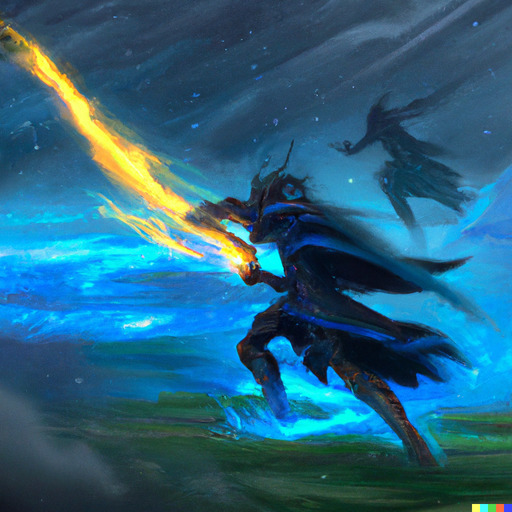
\includegraphics[width=\columnwidth]{core mechanics/spell and ritual mechanics}

    Spells and rituals share many common properties, defined here.

    % TODO: description
    \subsection{Categories of Magic}

    \subsubsection{Magic Sources}
        There are four \glossterm{magic sources} that characters can use to cast spells and perform rituals: arcane (cast by sorcerers and wizards), divine (cast by clerics and paladins), nature (cast by druids), and pact (cast by warlocks).
        Each magic source has a set of associated \glossterm{mystic spheres} (see Mystic Spheres, below).
        % TODO: more description

        \parhead{Characters with Multiple Magic Sources}
            A character can have access to multiple sources of magic through the use of abilities like the Hybrid Training ability (see \pcref{Half-Elves}).
            The \glossterm{mystic spheres}, spells, and rituals that character knows are tracked separately for each source of magic that character has access to.
            If you have access to the same spell or ritual from multiple sources, the two versions of the ability are generally considered to be the same ability.
            When you cast the spell or perform the ritual, you choose which source you are using for the ability.

        \subsubsection{Mystic Spheres}
            A \glossterm{mystic sphere} is a collection of thematically related magical effects that includes both \glossterm{spells} and \glossterm{rituals}.
            Each \glossterm{mystic sphere} can be associated with any number of \glossterm{magic sources}.
            The mystic spheres are listed at \pcref{Mystic Spheres}.

    \subsection{Ability Tags}
        All spells and rituals are \magical.
        In addition, all spells have the \abilitytag{Spell} \glossterm{ability tag}, and all rituals have the \abilitytag{Ritual} ability tag.
        Since spells and rituals are already clearly indicated in the Mystic Spheres chapter, the tags are omitted here to avoid unnecessary repetition.
        In some other places, such as monster descriptions, those tags may be used to indicate that specific abilities are considered spells or rituals despite not appearing in this chapter.

    \subsection{Casting Components}\label{Casting Components}
        Unless otherwise noted, all spells and rituals require \glossterm{verbal components} to cast or perform.
        In addition, spells and rituals from arcane and pact mystic sources require \glossterm{somatic components}.
        You cannot start casting a spell or performing a ritual without all required components.
        If you lose those components before the ability resolves, the spell fails with no effect.

        To provide the verbal component for a spell or ritual, you must speak in a strong voice with a volume at least as loud as ordinary conversation.
        To provide the somatic component for a spell or ritual, you must make a precise series of movements with at least one free hand.
        These movements involve your whole arm in addition to gestures with your fingers.

        \subsubsection{Somatic Component Failure}\label{Somatic Component Failure}
            Encumbrance from armor interferes with the \glossterm{somatic components} required to perform arcane spells, pact spells, and all rituals.
            When you cast a spell or perform a ritual that requires \glossterm{somatic components} while you have an \glossterm{encumbrance}, you must roll 1d10.
            If your result is less than or equal to your \glossterm{encumbrance}, the spell fails with no effect.
            When you perform a ritual, this roll must be repeated at the end of each round during the ritual.

    \subsection{Dismissal}\label{Dismissal}
        Many abilities can intentionally be ended early if you \glossterm{dismiss} it.
        When an ability is dismissed, all of its lingering effects immediately end.
        Unless otherwise noted, all \magical abilities with a duration can be dismissed, but \glossterm{mundane} abilities cannot be dismissed.
        This includes \glossterm{conditions}, \glossterm{brief} effects, and other abilities with more specific durations.
        You can dismiss abilities as a \glossterm{free action} that requires only mental effort.

    \subsection{Resurrecting the Dead}\label{Resurrecting the Dead}
        Several rituals have the power to restore dead characters to life.

        When a living creature dies, its soul departs its body, travels through the Astral Plane, and goes to abide on the plane where the creature's deity resides.
        If the creature did not worship a deity, its soul departs to the plane corresponding to its alignment.
        Bringing a creature back from the dead means retrieving their soul and returning it to their body.

        \parhead{Death and Old Age} While a creature is dead, it still tracks that time towards its maximum age.
        A creature's maximum age is largely determined by the strength of its soul, not the condition of its body.
        No magic can return a creature to life when it has passed its maximum age.

        \parhead{Preventing Resurrection} Enemies can take steps to make it more difficult for a character to be returned from the dead.
        Except for \spell{true resurrection}, every ritual to raise the dead requires a body, so keeping or destroying the body is an effective deterrent.
        The \spell{soul bind} ritual prevents any sort of revivification unless the soul is first released.

        \parhead{Involuntary Resurrection} A soul cannot be returned to life if it does not wish to be.
        A soul infallibly knows the name, alignment, and patron deity (if any) of the character attempting to revive it and may refuse to return on that basis.

    \subsection{Functioning Like Other Spells}\label{Functioning Like Other Spells}
        Many spells and rituals say they ``function like'' some other spell or ritual, often with some noted changes.
        Except as otherwise noted, they retain all of the original effects and targets of the spell.
        However, they do not have the same rank upgrades as the original spell or ritual.

    \subsection{Impossible Spells and Rituals}
        When you try to use a spell or ritual in an impossible way, the ability fails with no effect.
        This most commonly happens if you attempt to declare an invalid target for a spell.

    \subsection{Spells}\label{Spells}
        % TODO: better description
        A \glossterm{spell} is a discrete magical effect with a name, a \glossterm{rank}, and an effect.
        Each \glossterm{mystic sphere} has a number of spells associated with it.
        An ability that gives you access to \glossterm{mystic spheres} will define how many spells you know.
        A spell's \glossterm{rank} is the minimum \glossterm{archetype rank} you must have in the relevant spellcasting archetype to be able to learn and cast the spell.

        \subsubsection{Cantrips}\label{Cantrips}
            Some \glossterm{mystic spheres} have minor spells called cantrips.
            Anyone who has access to a mystic sphere knows all cantrips from that sphere.

    \subsection{Rituals}\label{Rituals}
        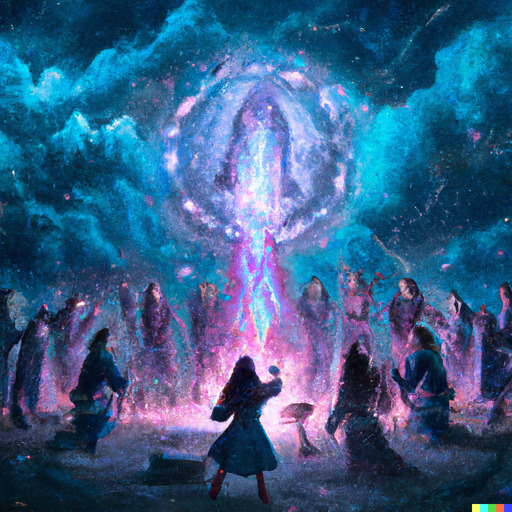
\includegraphics[width=\columnwidth]{core mechanics/rituals}

        Each \glossterm{mystic sphere} has a number of \glossterm{rituals}.
        Some spellcasting characters can learn and perform rituals.
        Rituals are ceremonies that create magical effects.
        Like spells, each ritual has a name, a \glossterm{rank}, and an effect.
        Although rituals are similar to spells, abilities that affect spells do not affect rituals unless they say they do in their descriptions.
        % Oddly located
        A ritual's \glossterm{rank} is the minimum \glossterm{archetype rank} you must have in the relevant spellcasting archetype to be able to learn and perform the ritual.

        You don't memorize a ritual as you would a normal spell.
        Rituals are too complex for all but the most knowledgeable sages to commit to memory.
        To perform a ritual, you need to read from a book or a scroll containing it.
        You must have access to the \glossterm{mystic sphere} a ritual is from in order to perform the ritual.

        \subsubsection{Ritual Descriptions}
            % TODO: proper chapter references
            Rituals are described in the body of the \glossterm{mystic sphere} they are associated with, following the description of spells from that mystic sphere.

        \subsubsection{Scribing Rituals}
            A ritual book contains one or more rituals that you can use as frequently as you want, as long as you can spend the time and \glossterm{fatigue level} to perform the ritual.
            Scribing a ritual costs precious magical ink with a value equal to an item of the ritual's rank (see \tref{Item Ranks}).

        \subsubsection{Performing Rituals}
            To perform a ritual, you must have a ritual book containing the ritual and the material components required for the ritual.
            Some rituals cause the creatures performing them to increase their \glossterm{fatigue level}, as indicated in their descriptions.
            Other creatures can suffer this fatigue to help you perform rituals; see Ritual Participants, below.

            % The fatigue level cost for 24 hour rituals is equal to (ritual rank ^ 2) * 2.
            % Should this be specified explicitly?

        \subsubsection{Ritual Participants}
            Creatures can assist in the performance of rituals even if they are unable to perform rituals themselves.
            A creature that helps perform a ritual is called a ritual participant, and the creature performing the ritual is called the ritual leader.
            A ritual participant may increase their \glossterm{fatigue level} in place of or in addition to the fatigue level gained by the creature performing the ritual.
            If multiple creatures are willing to increase their fatigue level or attune to effects, the ritual leader decides which creatures increase their fatigue level or attune to the ritual's effects.

            The steps required to participate in rituals can be complex.
            Ritual participants must be given specific instructions for the actions they must perform during a ritual by a creature who knows how to perform the ritual.
            This instruction generally takes one tenth of the time required to perform the ritual.
            A creature cannot participate in rituals unless it has an Intelligence of at least 0, can speak at least one language, and has the fine motor control required to perform the \glossterm{somatic components} of rituals.

            Normally, a ritual participant can only contribute \glossterm{fatigue levels} up to a maximum of their \glossterm{fatigue tolerance}.
            If the participant has access to the same \glossterm{magic source} as the ritual, they can contribute any number of \glossterm{fatigue levels} (until they drop unconscious).
            Creatures willing to fatigue themselves generally tire at a rate no faster than one fatigue level per ten minutes spent performing the ritual.

            \parhead{Changing Ritual Participation}
            Rituals are deeply complex magic, and they cannot be abandoned or paused partway through.
            If the number of ritual participants in a ritual decreases below its initial value, the ritual fails at the end of the next round if the number of participants is not restored.
            However, ritual participants can transfer their participation to other creatures without disrupting the ritual.

            In order to transfer ritual participation, the new creature must be able to participate in the ritual.
            Similarly, the ritual leader can transfer their leadership to another creature.
            In addition to the requirements for transferring ritual participation, the new leader must know the ritual and be able to perform it themselves.

            Changing ritual participation and leadership is usually done when performing extraordinarily long or demanding rituals.

            \parhead{Attunement Rituals}
                Rituals with the \abilitytag{Attune} tag require a single ritual participant to \glossterm{attune} to the ritual's effect.
                Any ritual participant can attune to the effect, but only one ritual participant can attune to the effect unless otherwise noted in the ritual's description.
                For details, see \pcref{Attuned Abilities}.

        \subsubsection{Magical Writings}
            To record a spell in written form, a character uses complex notation that describes the magical forces involved in the spell.
            The notation constitutes a universal language that spellcasters have discovered, not invented.
            Each writer uses this universal system regardless of their native language or culture.
            However, each character uses the system in their own way.
            Another person's magical writing remains incomprehensible to even the most powerful spellcaster until they take the time to study and decipher it.

\section{Common Magical Effects}
    \subsection{Delayed and Repeated Effects}\label{Delayed and Repeated Effects}
        Some abilities cause an effect to happen in a future round, or in all subsequent rounds.
        These abilities often say that they happen ``during your action''.
        When you act during each action phase, you can decide when that effect happens, including before and after all of your other actions.
        For example, you could resolve the trigger first to see the results before deciding your actions, or you could act before the trigger to push another creature into a relevant area.

        You must still complete all of your actions, including these triggers, as part of your single turn.
        You can't resolve a trigger, then let your allies take actions, then take your own action afterwards.

    \subsection{Resurrection}\label{Resurrection}
        Some abilities can return dead creatures to life.
        This is called resurrection.

        A creature has no hit points or damage resistance when it returns to life.
        It is cured of all \glossterm{vital wounds}, \glossterm{conditions}, and other negative effects, but the body's shape is unchanged.
        Any missing or irreparably damaged limbs or organs remain missing or damaged.
        The creature may therefore die shortly after being resurrected if its body is excessively damaged.
        Some resurrection abilities can restore more damaged corpses to life, as indicated in their descriptions.

        Coming back from the dead is an ordeal.
        The creature's maximum \glossterm{fatigue tolerance} is reduced by 1.
        This penalty lasts for thirty days, or until the creature gains a level.
        If this would reduce a creature's maximum fatigue tolerance below 0, the creature cannot be resurrected.

        Resurrection is always voluntary.
        If a dead creature's soul refuses to return to life, no effect can compel it to be resurrected.
        Similarly, if a dead creature's soul has been subsumed into the planar essence of its afterlife plane, it has already been resurrected, or the soul is otherwise inaccessible, resurrection is impossible.

        Although you can resurrect creatures who have died of old age, it is usually pointless.
        They will die again before long from some malady resulting from their advanced age.

    \subsection{Shapeshifting}\label{Shapeshifting}
        When a creature shapeshifts, its physical body completely transforms into a different shape.
        It generally retains all of its original statistics and abilities, with the following exceptions.
        Some specific abilities that cause a creature to shapeshift have additional effects.
        % TODO: are more exceptions necessary?
        \begin{itemize}
            \item The creature's size changes to match the new form.
                This can change the creature's \glossterm{base speed}, Reflex defense, and other statistics as normal (see \pcref{Size Categories}).
            \item The creature's \glossterm{mundane} movement modes and natural weapons are replaced with the movement modes and natural weapons of its new shape.
            \item If the new shape is not normally capable of speech, the creature cannot speak.
                This may prevent it from casting spells with \glossterm{verbal components} and using similar abilities.
            \item The creature is limited by the number of \glossterm{free hands} present in the new form.
                In addition, it cannot gain more free hands by shapeshifting than it originally had in its base form.
                Even if you shapeshift to a form with many hands, you do not have the mental coordination necessary to use them all effectively.
            \item Any special properties that a creature had that were originally a result of its pure physical composition may be lost.
                For example, a ghost would stop being \trait{incorporeal} if it shapeshifted.
        \end{itemize}

        All of a shapeshifted creature's equipment that is physically incompatible with the creature's new shape meld into its body.
        This does not break \glossterm{attunement}, and the creature still gains the benefit of any magical properties of melded items.
        However, it does not gain the benefit of nonmagical properties from melded items.
        For example, a creature that shapeshifts into an amorphous gas would still benefit from all attuned effects from its equipped items, such as \mitem{boots of speed}.
        However, it would gain no benefit to its Armor defense or damage resistance from any melded body armor, and it would not be able to attack with any of its melded weapons.
        Items exceeding a creature's \glossterm{carrying capacity} are not melded, and simply fall to the ground in place.

        When a shapeshifted creature dies, it returns to its original form.

    \subsection{Teleportation}\label{Teleportation}
        Some abilities can \glossterm{teleport} creatures or objects.
        When you are teleported, you move through the Astral Plane and arrive at a new location.
        You can be teleported between two different locations on the same \glossterm{plane}, or between two different locations on different planes.
        If for some reason you cannot access the Astral Plane, you cannot be teleported.

        Anything being teleported must have both \glossterm{line of sight} and \glossterm{line of effect} to its destination.
        In addition, the destination of the teleportation must be an unoccupied location on a stable surface that can support the weight of the teleporting creature or object.
        If either of these conditions is not met, the teleportation fails without effect.
        Some teleportation abilities are less restricted, as indicated in their description.

        In general, you can teleport up slopes that are no more than 45 degrees.
        Steeper slopes prevent you from seeing stable ground to teleport to it.
        The GM can provide guidance for individual slopes, which may be easier or harder to navigate with teleportation.

        \subsubsection{Teleportation Noise}\label{Teleportation Noise}
            Creatures and objects that are teleported make a sound when they depart and arrive.
            This noise is caused by the displacement of air (or other substances) created by the teleportation.
            The base \glossterm{difficulty value} of an Awareness check to hear this sound for a Medium creature or object is 10.
            This difficulty value changes based on the size of the teleported creature or object:

            \begin{itemize}
                \item Fine: 30
                \item Diminutive: 25
                \item Tiny: 20
                \item Small: 15
                \item Medium: 10
                \item Large: 5
                \item Huge: 0
                \item Gargantuan: \minus5
                \item Colossal: \minus10
            \end{itemize}

        \subsubsection{Carrying Objects}
            When a creature is teleported, it can bring along equipment and held objects as long as two conditions are met.
            First, the combined weight of the objects cannot exceed the creature's maximum \glossterm{carrying capacity} (see \pcref{Weight Limits}).
            If a creature is teleported while carrying more than its maximum carrying capacity, all excess objects are left behind, starting with the heaviest object and proceeding in order of weight.

            Second, no object can extend more than two feet away from the creature's body.
            Any objects that extend beyond that distance are left behind.
            For example, a creature wearing handcuffs will arrive at its teleportation destination still wearing the handcuffs.
            However, a creature that is tied to a post by a long rope will arrive at its teleportation destination without the rope.

        \subsubsection{Astral Beacon}\label{Astral Beacon}
            Some abilities allow long-distance teleportation, such as the \ritual{overland teleportation} ritual.
            This sort of teleportation is much easier if you are travelling to an \glossterm{astral beacon}.
            The specific effects of an astral beacon are defined in the teleportation ability being used.
            An astral beacon covers an area, rather than a single point in space.

            Each astral beacon has a unique name.
            The name represents the beacon's precise location in the Astral Plane, so no two beacons can have identical names.
            For example, astral beacons created by rituals have their name defined by the precise color of ritual inks, details of drawn patterns, timing and inflection of ritual incantations, and similar subtleties.

            It is possible, though unlikely, to find astral beacons simply by wandering in the Astral Plane.
            They are similar in size and shape to \glossterm{scrying sensors}, but their appearance is visually distinct (for creatures who can see \trait{invisible} objects).
            Inspecting a beacon can reveal the location it points to, and destroying the beacon in the Astral Plane removes the astral beacon entirely.
            This is generally considered a hostile act, and may have consequences.

        \subsubsection{Horizontal Teleportation}
            Some planes have a curved primary surface.
            On those planes, ``horizontal'' teleportation isn't objectively horizontal.
            Instead, it is horizontal relative to the surface of the plane.

\section{Breaking Objects}
    There are two main ways of breaking objects.
    You can deal damage to objects with attacks, similarly to how you can deal damage to creatures.
    Alternately, you can attempt to sunder the object with sheer strength.

    \subsection{Damaging Objects}
        Objects have \glossterm{hit points} and \glossterm{damage resistance} like creatures.
        However, non-creature objects treat all damage they take as \glossterm{environmental damage} (see \pcref{Environmental Damage}).
        That means that all damage they take is reduced by their \glossterm{damage resistance} without subtracting from the remaining value of their damage resistance.

        An object becomes \glossterm{broken} if its \glossterm{hit points} are reduced to 0 (see \pcref{Broken and Destroyed Objects}).
        Objects cannot gain \glossterm{vital wounds}.
        Objects are also not normally subject to \glossterm{critical hits}.

    \subsection{Sundering Objects}
        As a standard action, you can attempt to break an object with raw strength instead of damage.
        This requires two hands.
        When you sunder an object, make a Strength check.
        The \glossterm{difficulty value} of the check is equal to the object's \glossterm{damage resistance}, \plus5 for each \glossterm{weight category} above Diminuitive.

    \subsection{Broken and Destroyed Objects}\label{Broken and Destroyed Objects}
        An object that is reduced to 0 \glossterm{hit points} becomes \glossterm{broken}.
        You can destroy an object by causing it to lose additional hit points equal to ten times its maximum hit points, or by succeeding at a check to sunder the object by 10.

        \parhead{Broken Objects}\label{Broken Objects}
        Broken objects cannot be used for their intended purpose, but still retain enough of their original form to be repaired without too much work.
        For example, a broken wall lies in pieces on the ground and no longer blocks passage, but can be repaired with far less effort than would be required to create a wall from scratch.
        Magic items that are broken retain their magical properties once fixed.
        Broken (but not destroyed) objects can be repaired with the Craft skill (see \pcref{Craft}).

        \parhead{Destroyed Objects}\label{Destroyed Objects}
        Destroyed object have been damaged beyond hope of any sort of repair short of crafting the object again from raw materials.
        For example, a destroyed wall is reduced to dust or small, useless chunks of rubble.
        Magic items that are destroyed irrevocably lose their magical properties.
        The remains of a destroyed object generally occupy a space one size category smaller than the original object.
        Destroyed objects can be rebuilt with the Craft skill, but it requires significant time and investment.

    \subsection{Relative Damage Resistance}\label{Relative Damage Resistance}
        When an object would take damage from a \glossterm{strike}, if the \glossterm{damage resistance} of the attacking object or creature is lower than the damage resistance of the defender, the attacking object or creature takes the damage instead.
        For example, if you try to break a stone wall with a wooden club, the club will break instead of the wall.
        % TODO: define hardness for creatures and their natural weapons; natural weapons should generally have higher hardness than creatures to avoid hardness reflection being common

    \subsection{Breaking Equipment}\label{Breaking Equipment}
        Normally, a character's equipment cannot be damaged or otherwise affected by attacks.
        This includes worn items, anything held in your hands, and anything in a secure storage like a small backpack.
        Such items are considered \glossterm{attended}.
        They are unaffected by damage caused by area effects, and cannot be targeted individually.
        Some abilities can specifically target \glossterm{attended} objects, as indicated in their descriptions.

        \subsubsection{Loose Equipment}
            Some items are explicitly \glossterm{loose equipment}.
            Loose equipment does not gain the protections listed above while worn as equipment.
            It can be individually targeted by attackers, and is affected by area effects just like any other object in the area.

\section{General Calculations}

    \subsection{Stacking Rules}\label{Stacking Rules}
        Usually, modifiers stack with each other, meaning that you add or subtract all of the modifiers to get the final result.
        However, some modifiers do not stack with each other, as described below.
        When bonuses don't stack with each other, you only apply the largest bonus.
        Likewise, when penalties don't stack with each ather, you only apply the largest penalty.

        \parhead{Special Exceptions}

        \begin{itemize}
            \item Effects from the same source do not stack. Any ability with the same name has the same source.
            \item Magic bonuses do not stack with each other.
            \item If a creature gains the same condition multiple times, the effects do not stack, but each instance of the condition is tracked separately.
                The creature must remove all instances of the condition before the effects are removed.
            \item Multiple \magical effects that change a creature's \glossterm{size category} do not stack.
                If multiple magical effects both increase and decrease size, size increases offset size decreases on a one-for-one basis to determine the creature's final size.
            \item If you have two separate abilities which grant you a special sense with a particular range, such as \trait{darkvision} or \trait{blindsight}, you sum the range from both abilities to find your total range with that sense.
        \end{itemize}

    \subsection{Maximum Bonuses}\label{Ability Limits}
        Some bonuses specify that they cannot increase the value beyond a given point.
        These bonuses must always be applied last, and cannot be combined with other bonuses to exceed the maximum value.
        If multiple bonuses specify different maximum values, use the lower maximum value.
        If a bonus with a maximum value is applied to a value that already exceeds the maximum value the bonus can provide, simply ignore the bonus and its maximum value.

    \subsection{Doubling and Halving}\label{Doubling and Halving}
        If you double any in-game value twice, it becomes three times as large.
        An additional doubling would make it four times as large, and so on.
        Likewise, if you halve any in-game value twice, it becomes one-third as large.
        For example, if you have two different abilities that double your \glossterm{power} with an attack, you triple your power with that attack.

        This also applies to calculations using real-world values, such as movement and distance, as long as you're calculating the effects of abilities.
        For example, if you have two different abilities that double your range with a spell, your total range with that spell is three times the spell's normal range.

        \subsubsection{Doubling Damage}
            If you double your damage with a dice pool, you roll the same number of dice and modify the result.
            This is different from a \glossterm{critical hit}, which changes the number of dice you roll.
            As a result, if you get a \glossterm{critical hit} with a double-damage attack, you roll twice as many dice and then double the result, which typically means you deal 4x your normal damage.

    \subsection{Changing Statistics}

        Your modifiers and defenses can change for many reasons.
        In general, all changes take effect immediately.

        It is not normally possible for a character to lose access to resources that require them to make choices, such as insight points or trained skills.
        If a character does somehow lose the prerequisites for choices they have made, such as if their Intelligence is permanently reduced, they immediately lose relevant abilities until they are within their new limits.

    \subsection{Rounding}
        In general, if you encounter a fractional number, you round it down.
